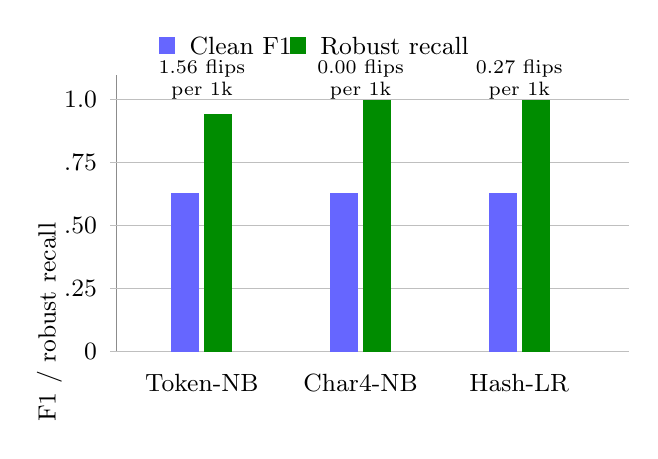
\begin{tikzpicture}[
  x=1.55cm,
  y=3.2cm,
  font=\small
]
\draw[black!45] (0,0) -- (4.2,0);
\draw[black!45] (0,0) -- (0,1.1);
\foreach \y/\label in {0/0,0.25/.25,0.5/.50,0.75/.75,1/1.0} {
  \draw[black!25] (-0.05,\y) -- (4.2,\y);
  \node[anchor=east] at (-0.08,\y) {\label};
}
\node[anchor=east, rotate=90] at (-0.55,0.55) {F1 / robust recall};

% Token-NB
\fill[blue!60] (0.45,0) rectangle (0.68,0.631);
\fill[green!55!black] (0.72,0) rectangle (0.95,0.944);
\node[anchor=north] at (0.70,-0.05) {Token-NB};

% Char4-NB
\fill[blue!60] (1.75,0) rectangle (1.98,0.630);
\fill[green!55!black] (2.02,0) rectangle (2.25,1.000);
\node[anchor=north] at (2.00,-0.05) {Char4-NB};

% Hash-LR
\fill[blue!60] (3.05,0) rectangle (3.28,0.630);
\fill[green!55!black] (3.32,0) rectangle (3.55,0.999);
\node[anchor=north] at (3.30,-0.05) {Hash-LR};

\fill[blue!60] (0.35,1.18) rectangle (0.48,1.25);
\node[anchor=west] at (0.52,1.215) {Clean F1};
\fill[green!55!black] (1.42,1.18) rectangle (1.55,1.25);
\node[anchor=west] at (1.59,1.215) {Robust recall};

% flip-rate callouts per 1000 variants
\node[align=center, font=\scriptsize] at (0.70,1.08) {1.56 flips\\per 1k};
\node[align=center, font=\scriptsize] at (2.00,1.08) {0.00 flips\\per 1k};
\node[align=center, font=\scriptsize] at (3.30,1.08) {0.27 flips\\per 1k};
\end{tikzpicture}
